\chapter{Tribal NeuroSim: Experimental Runs and Results}

\section{World Mechanics}

The simulation space is a hexagonal grid. Runs initialised from the flexset dataset take place on a map of approximately 36\,100 tiles; soloq runs receive smaller worlds. Each tile is assigned a biome type (DenseForest, Riverland, DrySteppe, Mountains, Marsh, Cold) that determines its base food production rate.

Tribes evolve through five polity levels: \textit{Wandering Band}, \textit{Settled Village}, \textit{Chiefdom}, \textit{Kingdom}, and \textit{Empire}. Each level-up requires meeting population, territory, and alliance thresholds; higher levels unlock greater maximum population and better combat efficiency, but also impose higher food-maintenance demands. Reaching Empire level is the victory condition: all four full runs and every run in the 103-seed sweep concluded with an Empire-level winner.

Combat outcomes are based on a Poisson process: the population sizes and combat artifacts of the opposing parties influence the expected casualties, but the concrete tick-level outcome is stochastic. The \textit{liveness-fix} corrected a determinism bug: unordered iteration over clusters produced different tick orderings and therefore different outcomes; after introducing \textit{sort\_by(id)}, re-runs produce bit-identical results. Detailed advancement conditions and iterative design decisions can be found in the extended version \cite{premadegraph-full}.

\section{Summary of the Four Runs}

Summary of the four full experimental runs:

\begin{table}[h]
\centering
\small
\caption{Comparison of the four final Tribal NeuroSim runs}
\label{tab:neurosim-run-comparison-final}
\resizebox{\textwidth}{!}{%
\begin{tabular}{|l|l|l|l|l|l|l|l|}
\hline
\textbf{Run} & \textbf{Dataset} & \textbf{Seed} & \textbf{Winner} & \textbf{Behaviour} & \textbf{Aggression} & \textbf{Migration} & \textbf{Final tick} \\
\hline
run67fl7777 & Flexset & 7777 & Tribe 355 & Warband/Combat & 0{,}18 & 0{,}88 & 2538 \\
run67fl42 & Flexset & 42 & Tribe 596 & Warband/Combat & 0{,}13 & 0{,}87 & 2487 \\
run67sq42 & SoloQ & 42 & Tribe 89 & Vanguard/Risk & 0{,}11 & 0{,}16 & 2046 \\
run67sq7777 & SoloQ & 7777 & Tribe 70 & Supply/Resource & 0{,}68 & 0{,}87 & 2541 \\
\hline
\end{tabular}
}
\end{table}

\begin{figure}[H]
\centering
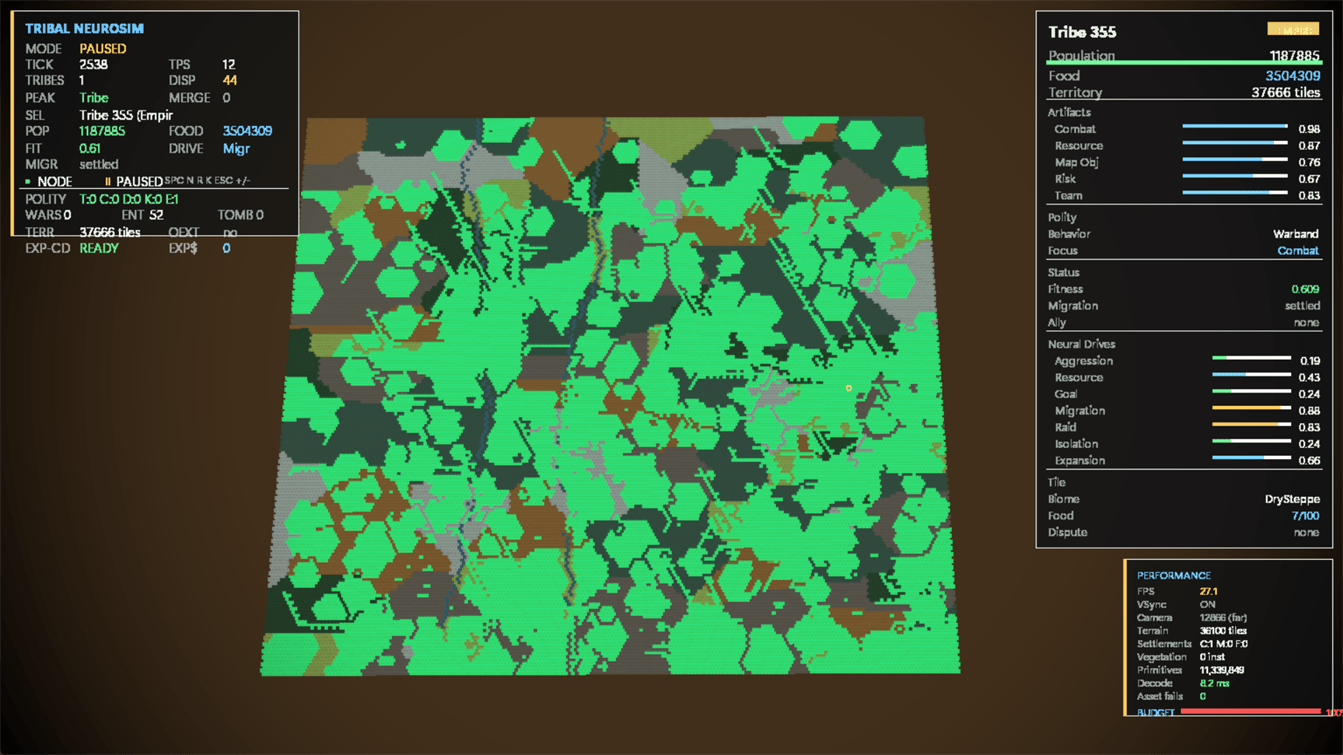
\includegraphics[width=0.9\textwidth]{assets/neurosim/run67fl7777-fl-s7777-tick2538-last.png}
\caption{Flexset, seed=7777, tick=2538: Tribe 355 (Warband/Combat) victory, final territory 37\,666 tiles.}
\end{figure}

\begin{figure}[H]
\centering
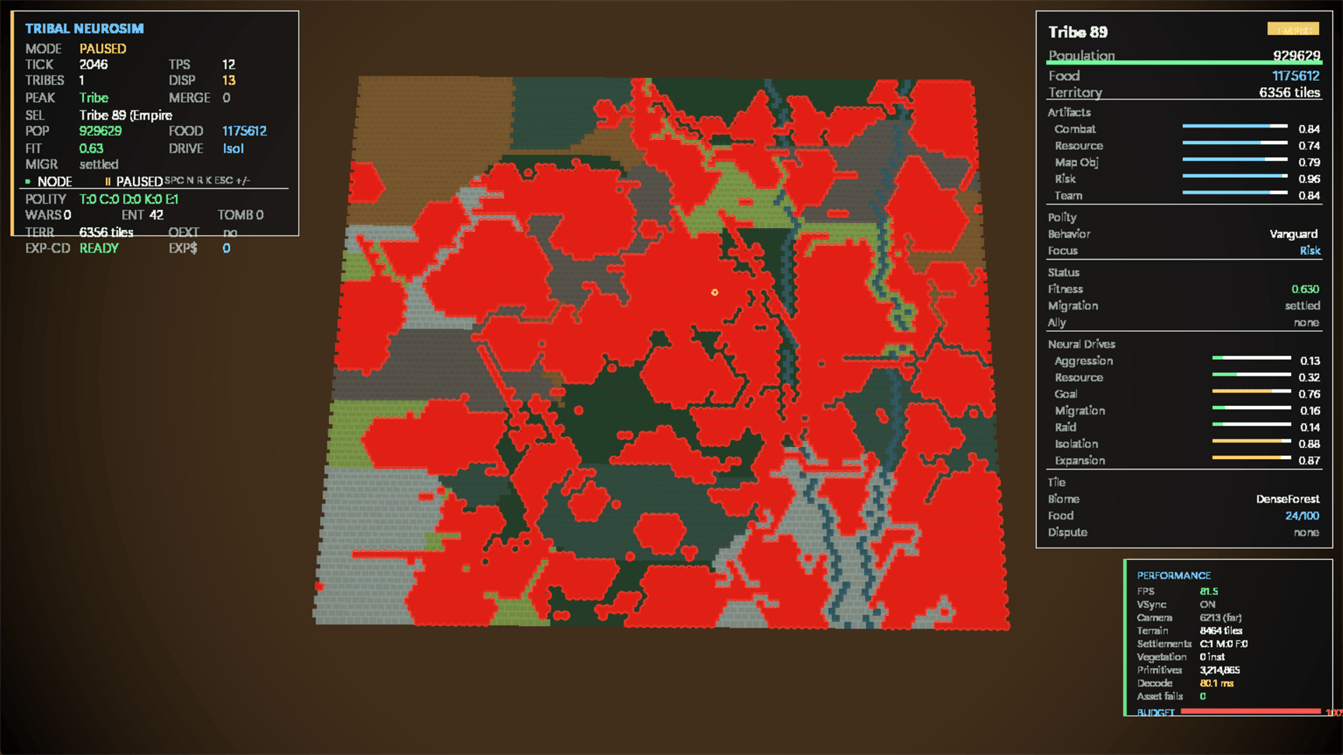
\includegraphics[width=0.9\textwidth]{assets/neurosim/run67sq42-sq-s42-tick2046-last.png}
\caption{SoloQ, seed=42, tick=2046: Tribe 89 (Vanguard/Risk) victory, final territory 6\,356 tiles.}
\end{figure}

\begin{figure}[H]
\centering
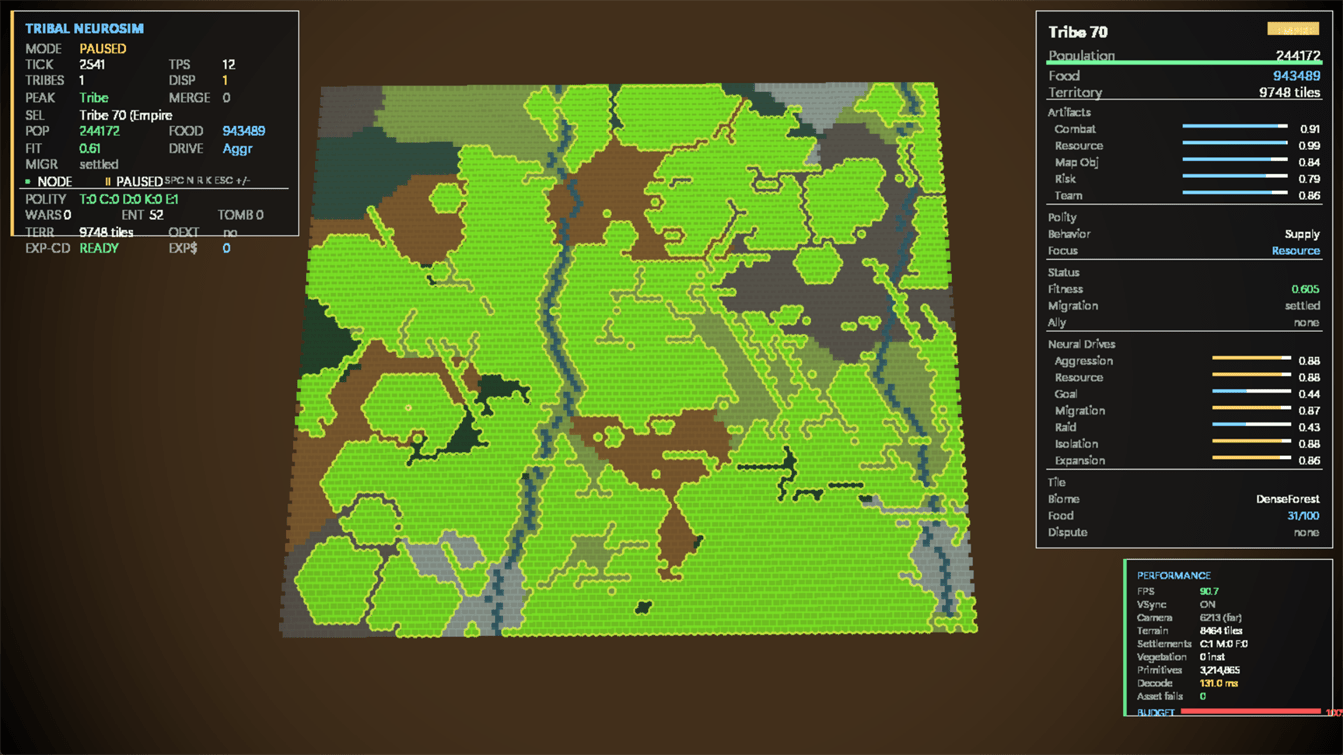
\includegraphics[width=0.9\textwidth]{assets/neurosim/run67sq7777-sq-s7777-tick2541-last.png}
\caption{SoloQ, seed=7777, tick=2541: Tribe 70 (Supply/Resource) victory, final territory 9\,748 tiles.}
\end{figure}

\section{103-Seed Sweep and Winner Archetype Distribution}

The four experimental runs are supplemented by a 103-seed soloq sweep. Every run in the sweep concluded with an Empire-level winner (103/103). Archetype distribution:

\begin{table}[H]
\centering
\caption{Winner archetype distribution across the soloq 103-seed sweep}
\label{tab:soloq-sweep-archetypes}
\begin{tabular}{|l|r|r|}
\hline
\textbf{Archetype} & \textbf{Runs} & \textbf{Share} \\
\hline
Warband   & 36 & 35{,}0\% \\
Supply    & 23 & 22{,}3\% \\
Council   & 20 & 19{,}4\% \\
Vanguard  & 14 & 13{,}6\% \\
Pathfinders & 10 & 9{,}7\% \\
\hline
\textbf{Total} & 103 & 100\% \\
\hline
\end{tabular}
\end{table}

The average finishing tick is 2308{,}57; the average winner territory is 8\,338 tiles. The Warband archetype leads with a slight plurality (35\%) but does not hold strong, seed-independent dominance.

\section{What the Results Show}

Both tested flexset runs (seed=42 and seed=7777) ended in a Warband/Combat profile victory, with low aggression (0{,}13--0{,}18) and high migration (0{,}87--0{,}88). The soloq runs produced more variable winner profiles: seed=42 produced a Vanguard/Risk winner, seed=7777 a Supply/Resource winner.

This difference is interpretable from the underlying graph structure. The flexset dataset carries more organised, recurring connection patterns, while the soloq dataset captures more individual performance profiles without persistent co-queue structure.

The interpretation is correlational, not causal. Correctness was verified through deterministic batch validation: in five parallel headless runs of flexset seed=42, Tribe 596 (Warband/Combat) won every time, with bit-identical \textit{final\_summary} records.

Under identical rule conditions, \textit{flexset} priors produced a Warband/Combat winner for both seeds (aggression 0{,}13--0{,}18), while \textit{soloq} priors produced a different archetype per seed (Vanguard and Supply respectively) --- the initial cluster prior measurably changes the outcome. The results do not demonstrate actual player psychology and do not predict outcomes of real League of Legends matches.
